\documentclass[a4paper, 11pt]{report} %twoside
\title{Programación, Redes y Código Libre}
\author{David Davó}
\date{\today{}}

%%Packages
\usepackage[utf8]{inputenc} %Para saber el encoding del archivo
\usepackage[T1]{fontenc}
%\usepackage[no-math]{fontspec} %Para usar fuentes del sistema
\usepackage{fontspec}

\usepackage[xindy, nomain, acronym, nonumberlist, nopostdot]{glossaries}
\usepackage{glossary-mcols}

\usepackage[ampersand]{easylist} %Cosas de listas

\usepackage{graphicx} %Para insertar gráficos
\usepackage{float} %PAra posicionar bien los gráficos
\usepackage{unicode-math} %Para símbolos matemagicos
%\setmathfont{Asana-Math.otf}
\setmathfont{Arial}
\usepackage[type={CC}, modifier={by-sa}, version={4.0}]{doclicense} %Muestra la licencia
\usepackage[usenames,svgnames,table]{xcolor} %Para darle color
\usepackage{dirtytalk} %Usado para citar
\usepackage{fvextra}
\usepackage{csquotes} %lo mismo qu eel anterior pero con estilo
\usepackage[spanish]{babel} %Hace que el idioma de los defaults esté en Español
\usepackage{fancyhdr} %Para poner encabezados y pies de página
%De la bibliografía y las citas.
\usepackage[
backend=biber
]{biblatex}
\addbibresource{Bibl.bib}

%Decoraciones y formato del texto
\usepackage[left=2.75cm, right=2cm, top=3cm, bottom=3cm]{geometry}

\usepackage[cache=false]{minted} %Para insertar código

\usepackage{tabularx} %Para hacer tablas muy bonicas
\usepackage{multirow}

\setmainfont{Arial}
\setmonofont{Inconsolata}
\fontsize{11}{14}
%Pies de pagina y eso
\pagestyle{fancy}
\fancyhf{}
\makeatletter
\fancyhead[LE, RO]{\@author}
\fancyhead[RE, LO]{\@title}
\fancyfoot[LE, RO]{\thepage}
\fancyfoot[C]{\leftmark}

\makeglossaries
\newglossaryentry{Libr}
{
	name=Librería,
	description={En informática, una librería o biblioteca es un conjunto de recursos y fucniones diseñadas para ser usadas por otros programas. Incluyen plantillas, funciones y clases, subrutinas, código escrito, variables predefinidas...},
	plural=librerías,
}
\newglossaryentry{datos}{
	name=Datos,
	description={Secuencia binaria de unos y ceros que contiene información codificada},
	plural=Datos, 
}
\newacronym{gnu}{GNU}{\textit{GNU's Not Unix} (GNU no es Unix)}
\newglossaryentry{Linux}
{
  name=Linux,
  description={is a generic term referring to the family of Unix-like
               computer operating systems that use the Linux kernel},
  plural=Linuces
}
\newglossaryentry{conmutacion de paquetes}{
	name={Conmutación de paquetes},
	description={Método para enviar datos por una red de computadoras. Se divide el paquete en dos partes, una con información de control que leen los nodos para enviar el paquete a su destino y los datos a enviar},
}
\newacronym{osi}{OSI}{\textit{Open Systems Interconnection} (Interconexión de Sistemas Abiertos)}
\newglossaryentry{gls-ISO}{
	name={\textit{International Organization for Standardization}},
	description={Organización Internacional de Normalización. Compuesta de varias organizaciones nacionales se encarga de la creación de estándares internacionales desde 1947.},
}
\newacronym[see={[Glossary:]{gls-ISO}}]{iso}{ISO}{\textit{International Organization for Standardization}\glsadd{gls-ISO}}
\newglossaryentry{capas de abstraccion}{
	name={capas de abstracción},
	description={Método de ocultar detalles de implementación de un set de funcionalidades},
}
\newacronym{IEEE}{IEEE}{Instituto de Ingeniería Eléctrica y Electrónica}
\newglossaryentry{topologia de red}{
	name={topología de red},
	description={Configuración espacial o física de la red. (Ver \ref{topdred} pág.\pageref{topdred})},
	plural={topologías de red},
	see={topologia}
}
\newglossaryentry{topologia}{
	name={topología},
	description={``Rama de las matemáticas que trata especialmente de la continuidad y de otros conceptos más generales originados de ella, como las propiedades de las figuras con independencia de su tamaño o forma." \cite{rae}[Topología]},
	plural={topologías},
}
\newglossaryentry{hardware}{
	name={hardware},
	description={Conjunto de elementos físicos o materiales que constituyen un sistema informático.},
}
\newacronym{MAC}{MAC}{\textit{Media Access Control}, Control de Acceso al Medio}
\newacronym{ADSL}{ADSL}{\textit{Asymmetric Digital Subscriber Line} [Línea de Abonado Digital Asimétrica]}
\newacronym{LAN}{LAN}{\textit{Local Area Network} [Red de Área Local]}
\newacronym{FTTH}{FTTH}{\textit{Fiber To The Home} [Fibra hasta el hogar]}
\newacronym[see={[Glossary:]{gls-FTTx}}]{FTTx}{FTTx}{\textit{Fiber to the X \glsadd{gls-FTTx}}}
\newglossaryentry{gls-FTTx}{
	name={FTTx},
	description={Término que agrupa las distintas configuraciones de acometida de la fibra óptica.},
}
\newglossaryentry{bit}{
	name={bit},
	description={\textit{\textbf{Bi}nary digi\textbf{t}, o dígito binario. Cada dígito del sistema de numeración binario}},
	plural={bits}
}
\newacronym{POP3}{POP3}{\textit{Post Office Protocol}, Protocolo de Oficina Postal}
\newacronym{url}{URL}{\textit{Uniform Resource Identifier}, Identificador de Recursos Uniforme}
\newglossaryentry{cache}{
	name={caché},
	description={Almacenamiento temporal de datos con el objetivo de reducir el retardo, la carga de los servidores y el ancho de banda consumido},
}
\newglossaryentry{programacion imperativa}{
	name={programación imperativa},
	description={Las órdenes del programa cambian el estado de este mismo. Por ejemplo, una variable no tiene por que ser declarada con antelación y su valor es modificable. Es la que usa el código máquina de los ordenadores},
}
\newglossaryentry{botnet}{
	name={botnet},
	description={Grupo de ordenadores coordinados conectados a un maestro mediante un virus. Gracias a este virus se pueden realizar tareas masivas como el envío de SPAM o ataques DDoS},
}
\newglossaryentry{bug}{
	name={bug},
	plural={bugs},
	description={Error en un programa informático.},
}
\newglossaryentry{repositorio}{
	name={repositorio},
	plural={repositorios},
	description={Servidor donde se alojan ficheros o archivos para su descarga},
}
\newglossaryentry{dependencia}{
	plural={dependencias},
	name={dependencia},
	description={De un programa, otro tipo de software necesario para que éste funcione}
}
\newacronym{FSF}{FSF}{\textit{Free Software Foundation}, Fundación del Software Libre}
\newacronym{IDE}{IDE}{Entorno de Desarrollo Integrado, \textit{Integrated Development Enviroment}}
\newacronym{GUI}{GUI}{Interfaz Gráfica de Usuario, \textit{Graphic User Interface})}

%%% Algunas macros
\newcommand{\acr}[1]{\acrshort{#1} (\acrlong{#1})}
\DeclareFontShape{EU1}{Inconsolata(0)}{bx}{n}{<->ssub*Inconsolata(0)/m/n}{}

%Document
\begin{document}
\makeatletter
\begin{titlepage}
\centering
\vspace*{4cm}
{\scshape\LARGE IES Palas Atenea \par}
\vspace{1cm}
{\scshape\Large Proyecto de Investigación Bachillerato de excelencia\par}
\vspace{1.5cm}
{\huge\bfseries \@title\par}
\rule{0.5\textwidth}{1pt}\par
\vspace{2cm}
{\Large\itshape \@author\par}
\vfill
Tutor\par
Julio Sánchez

\vfill

{\large \@date\par}
\pagenumbering{gobble}
\end{titlepage}
\clearpage

\tableofcontents
\newpage{}
\pagenumbering{arabic}

\chapter{Programación y código libre}

\textbf{\texttt{\f@family{}, \f@series{}, \f@shape{}, \f@size{}}}

\subsection*{Propuesta}
El objetivo es el desarrollo de un software programado en Python de código libre con el que los alumnos puedan aprender tanto sobre redes como de programación en Python.

\section{Herramientas}
El programa ha sido creado con herramientas de software libre. Según la Free Software Foundation
\say{«Software libre» es el software que respeta la libertad de los usuarios y la comunidad. A grandes rasgos, significa que los usuarios tienen la libertad de ejecutar, copiar, distribuir, estudiar, modificar y mejorar el software. Es decir, el «software libre» es una cuestión de libertad, no de precio. Para entender el concepto, piense en «libre» como en «libre expresión», no como en «barra libre». En inglés a veces decimos «libre software», en lugar de «free software», para mostrar que no queremos decir que es gratuito.}
--\cite{FSF-Ph}

Todas las herramientas citadas a continuación, son o están basadas en Software Libre.

\subsection{GNU/Linux}
También llamado incorrectamente sólo Linux, es una manera de llamar al Sistema Operativo (OS) combinación del kernel Linux (Basado en Unix) y el OS \gls{gnu}, ambos software son libres y de código abierto. Normalmente Linux se distribuye en distribuciones o 'distros', las cuales contienen paquetes de software preinstalados, dependiendo del grupo de usuarios al que este dirigida.

\subsubsection*{Distros}

\subsection{Git y Github}
Git es un software diseñado por Linus Torvalds con el que puedes crear un Sistema de
Control de Versiones o VCS (\textit{Version Control System}). Este programa te permite
de forma sencilla volver a una versión o \textit{commit} anterior del programa, así
como enviarlas a un repositorio remoto e incluso publicarlas en línea. Su punto fuerte
son las \textit{branches} o ``ramificaciones" del código, haciendo que la rama
\textit{master} (principal) siempre pueda ser usada. Para ello creamos una nueva rama
para cada nueva funcionalidad del programa. La implementación del nuevo código a otra
rama se denomina \textit{merge}.

%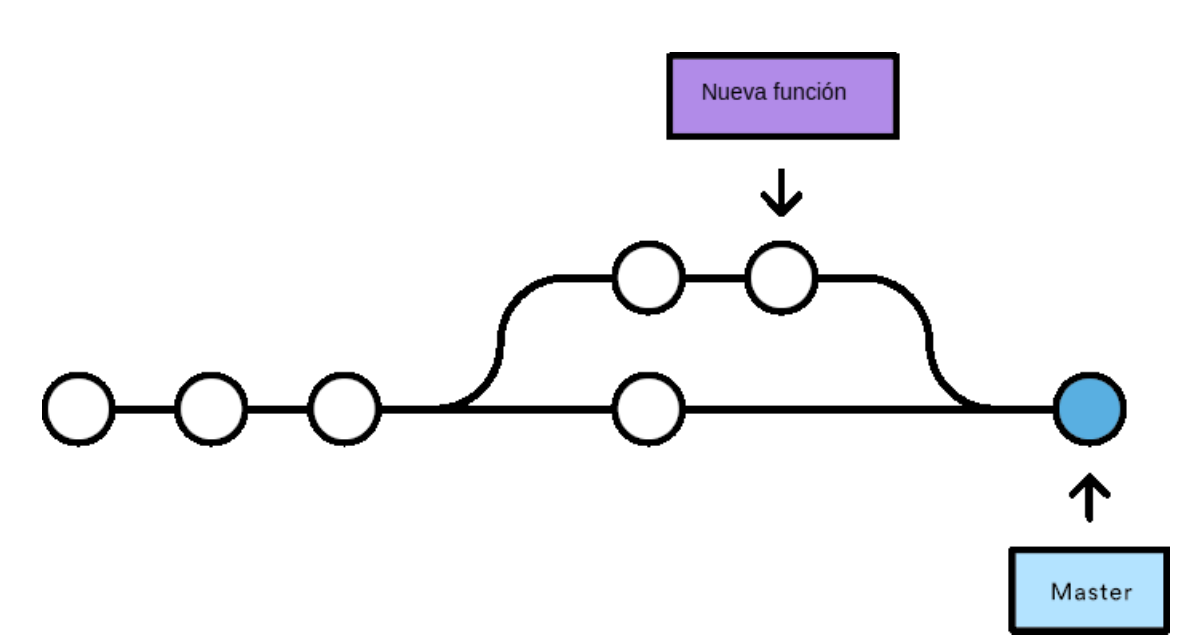
\includegraphics[width=\textwidth]{Resources/01.01.02-01.png}
\begin{figure}
\noindent
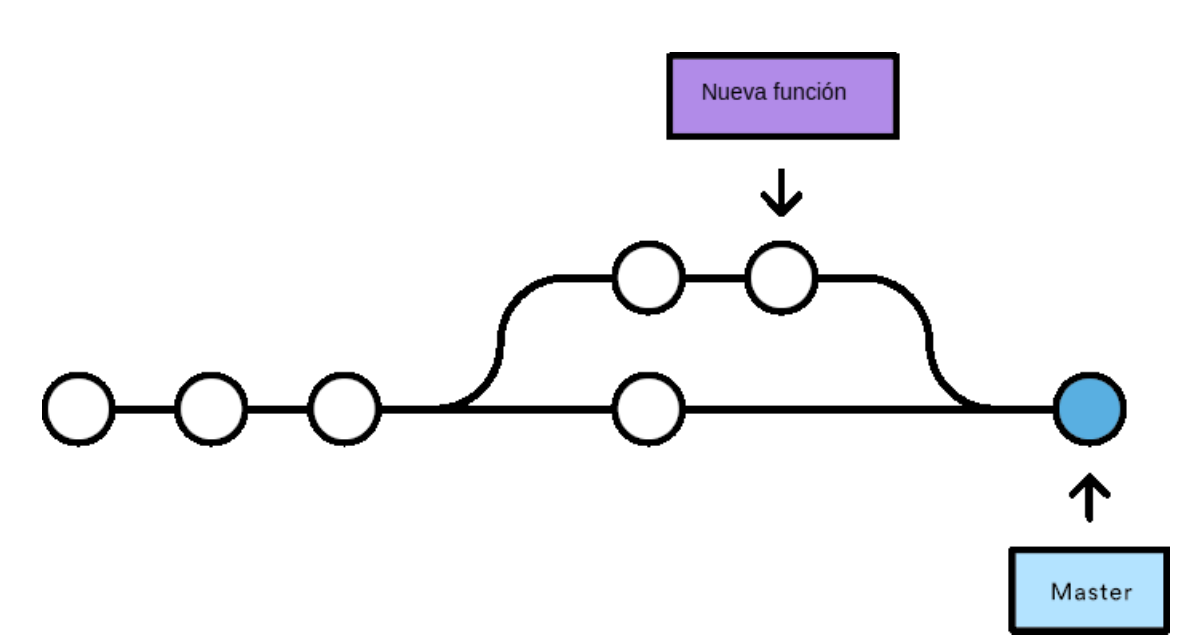
\includegraphics[width=0.95\textwidth]{Resources/01.01.02-01.png}
\caption{\textit{Branching} con Git}
\end{figure}

GitHub es una plataforma de desarrollo colaborativo que te permite alojar tus repositorios Git. Su uso es gratuito si el código almacenado es público. Además, te permite tener, una wiki y una página web para tu proyecto, junto a otras funciones.
Tanto el programa como este documento están disponibles en GitHub en el siguiente enlace. \url{https://github.com/daviddavo/InvProy}

\subsection{LaTeX}
\LaTeX\space o, en texto plano, LaTeX, pronunciado con la letra griega 
Ji ($\Chi$), es un software libre orientado a la creación de textos escritos comparable a la calidad tipográfica de las editoriales. Mediante la importación de paquetes y comandos o macros se puede dar formato al texto al igual que con cualquier otro editor, exportándolo posteriormente a PostScript o PDF. Está orientado a documentos técnicos y científicos por su facilidad a la hora de incluir fórmulas e importar paquetes que cumplan tus necesidades. No es un procesador de textos, pues está más enfocado en el contenido del documento que en la aparencia de éste.
El código del documento puede ser editado con cualquier editor de texto plano como \textit{nano} o \textit{emacs}, pero he usado una IDE llamada \textbf{texmaker}.

\subsection{Python}
Es un lenguaje de programación interpretado (sólo traducen el programa a código máquina cuando se debe ejecutar esa parte del código, por lo que no hace falta compilarlo) que destaca por pretender una sintaxis más legible que la de el resto de lenguajes. Soporta tanto \gls{programacion imperativa} como programación orientada a objetos. Usa variables dinámicas, es multiplataforma, y, además, es de código abierto, lo que me permite distribuir el programa en Windows al distribuir los binarios de Python junto a él. En este caso, la versión de Python usada es la 3.4 en adelante.

\subsection{Gtk+}
Es un conjunto de bibliotecas o \glspl{Libr} (conjunto de funciones y clases ya definidas preparadas para el uso de los programadores) desarrollado por la GNOME foundation destinado a la creación de GUIs (Interfaz Gráfica de Usuario), también, al igual que Linux forma parte del proyecto GNU.

Contiene las bibliotecas de GTK, GDK, ATK, Glib, Pango y Cairo; de las que he usado fundamentalmente GTK para crear la interfaz principal del programa; GDK al usarlo como intermediario entre los gráficos de bajo nivel y alto nivel y Cairo para la creación de algunos de los elementos gráficos del programa.

Al usar este conjunto de librerías, he conseguido que sólo sea necesario descargar una dependencia del programa, que además suele venir instalada en la mayoria de distros de Linux, por ejemplo en una instalación limpia de Ubuntu 16 (sin descargar paquetes adiccionales) el programa funciona perfectamente. Para usarlo en Python se ha tenido que importar la libreria de PyGtk.
\subsection{Atom}
Atom es un editor de código multiplataforma con soporte para plugins escrito en Node.js, también tiene soporte para Git. También es un programa de código libre haciendo uso de la licencia MIT.

\subsection{Wireshark}
\label{wireshark}
Wireshark es un \textit{packet sniffer} o analizador de paquetes. Te muestra los paquetes de red reales enviados y recibidos por una tarjeta de red, lo que facilita la creación del simulador de redes. También te separa las distintas partes de la encapsulación del paquete.

\chapter{Redes Informáticas}
\section*{Historia}
Internet, tal y como lo conocemos ahora, haciendo uso de IPv6, HTML5, CSS3 no existe hasta hace poco, pero el desarrollo de éste transcurre desde los años 60. En 1961 se publican los primeros artículos de \gls{conmutacion de paquetes}
\section{Capas de Red/Modelo OSI}
El modelo \acr{osi} es un modelo de referencia para redes basado en \gls{capas de abstraccion}.
El objetivo del modelo \acrshort{osi} es conseguir la interoperabilidad entre sistemas con la protocolos estandarizados. Fue creado en 1980 por la \acr{iso}. No es considerado una arquitectura de red porque los protocolos no forman parte del modelo, sino son entidades de distintas normativas internacionales.
\definecolor{odd}{HTML}{FFFFFF}
\definecolor{even}{HTML}{E0E0E0}
\definecolor{header}{HTML}{42A5F5}

\rowcolors{1}{header}{header}
\rowcolors{2}{odd}{even}
\renewcommand{\arraystretch}{1.1}
\noindent
\begin{tabularx}{\linewidth}{ | l c X p{2cm} | }
	\rowcolor{header} \hline
	\textbf{Capa} & \textbf{PDU\footnote{\textit{Protocol Data Unit} o Unidad de Datos de Protocolo.}} & \textbf{Función} & \textbf{Ejemplos} \\ \hline
	1. Física & Bit & Transmisión y recepción de bits físicos sobre un medio físico (topología de red) & 	 RJ45, IEEE 802.11, etc. \\
	\label{osi}
	2. Data Link & Frame & Transmisión segura de \textit{frames} entre dos nodos conectados por una capa física. & Ethernet, 802.11, etc...\\
	3. Red & Paquete & Estructurar y administrar una red multinodo. Incluye enrutamiento, control de tráfico, y asignación de direcciones & IPv4, IPv6, ICMP... \\
	4. Transporte & \begin{tabular}[t]{@{}c@{}}Datagrama(UDP)\\Segmento(TCP)  \end{tabular} &
	Transmisión de segmentos de datos entre los puntos de una red, incluyendo ACK & TCP, UDP...\\
	5. Sesión & Datos & Administración de sesiones de comunicación, como intercambio continúo de información entre dos nodos. & SSH, RPC, PAP...\\ 
	6. Presentación & Datos & Translación de datos entre un servicio de red y una aplicación. Incluye comprensión, encriptación/decriptación, y codificación de carácteres. & MIME, TLS \\
	7. Aplicación & Datos & APIs de alto nivel, incluyendo recursos compartidos y acceso remoto de archivos & HTTP, FTP, SMTP... \\ \hline
\end{tabularx}

\section{Elementos físicos de una red}
Servidor, cliente, switch, hub, router, etc...

\section{Topologías de red}
\label{topdred}
La \gls{topologia} de red es la configuración de los elementos que componen una red. Puede ser representada lógica o físicamente. La topología lógica puede ser igual en dos redes, aunque su topología física (distancia entre conexiones, tipo de señales...) pueda ser distinta. Se distinguen dos elementos: los nodos (Ordenadores, switches, etc.) y los enlaces (medio de transmisión de los datos).
\subsection{Clasificación de las topologías de red}
Se distinguen ocho tipos de topologías de red: \cite{bicsi-02}
\begin{description}
\item \textbf{Punto a punto:} conexión directa entre los dos puntos de la red. También es conocida como \textit{P2P} (\textit{Peer to Peer}).
\item \textbf{Estrella:} cada host se conecta a un hub central con una conexión P2P. Cada nodo está conectado a un nodo central que puede ser un router, hub o switch.
\item \textbf{Bus:} cada nodo está conectado a un sólo cable. Una señal de un dispositivo viaja en ambos sentidos por el cable hasta que encuentra el destino deseado.
\item \textbf{Anillo:} es una topología en bus pero con los extremos conectados. Los datos atraviesan el anillo en una única dirección y van atravesando cada uno de los nodos, por lo que si uno de ellos no funciona, la red tampoco.
\item \textbf{Malla:} se pueden distinguir dos tipos: completamente conectados, en la que todos los nodos están conectados entre ellos y parcialmente conectados, en la que algunos nodos pueden estar conectados punto a punto y otros pueden tener varias conexiones.
\item \textbf{Híbrida:} combinan dos o más topologías. La más famosa es la topología de \textbf{árbol}, en la que se conectan varias topologías de estrella mediante bus. 
\item \textbf{Cadena:} se conecta cada ordenador en serie con el siguiente. Cada ordenador repite el mensaje al siguiente ordenador si éste no es su destino. Si se cierra el circuito se crea una topología en anillo, mientras que si se deja abierto se denomina topología linear.
\end{description}

\subsection{Nodos de una red}
\begin{description}
\item \textbf{\textit{Router} o enrutador:} es un dispositivo de red que reenvía los paquetes mirando en la capa 3 del modelo OSI (IP) y conecta dos redes.
\item \textbf{Puente de red o \textit{bridge}:} Funciona en la capa 2 del modelo OSI. Es un dispositivo que conecta dos segmentos de red formando una única subred, por lo que las dos ``redes" pueden conectarse e intercambiar datos sin necesidad de un \textit{router}.
\item \textbf{Conmutadores o \textit{switches}:} dispositivo de red que filtra los datagramas del nivel 2 OSI (\textit{Data Link Layer}, ver \ref{osi}, pág. \pageref{osi}), también conocidos como \textit{frames}, y reenvía los paquetes recibidos entre los puertos, dependiendo de la dirección MAC de cada \textit{frame}. La diferencia entre un \textit{switch} y un \textit{hub} es que el \textit{switch} sólo reenvía los paquetes por el puerto necesario. También existen un tipo especial de \textit{switches} que pueden mirar en el nivel 3 OSI.
\item \textbf{Repetidores y hubs:} un repetidor es un dispositivo de red que, llegada una señal, limpia el ruido innecesario y la regenera. Un repetidor con múltiples puertos es un hub, trabajan en la capa 1 del modelo \acr{osi}. Los repetidores requieren un pequeño tiempo para regenerar la señal, lo que puede crear un retardo en la señal.
\item \textbf{Interfaces de Red:} también conocido como tarjeta de red o \textit{Network Interface Controller} (NIC), es un \gls{hardware}, normalmente integrado en la placa base, que permite al ordenador conectarse a una red. Recibe el tráfico de una dirección de red. En las redes de Ethernet, tiene una dirección \acr{MAC} única. Estas direcciones son administradas por el \acr{IEEE} evitando la duplicidad de estas. Cada dirección MAC ocupa 6 octetos, o 48 bits, a lo que suele ser representada como una cadena hexadecimal, por ejemplo: ``43:31:50:30:74:33".
\item \textbf{Módem:} Dispositivos que transforman señales analógicas a digitales y viceversa. Son usados mayoritariamente en el \acr{ADSL}.
\item \textbf{Cortafuegos o \textit{firewalls}:} dispositivo que controla la seguridad mediante reglas de acceso. Aceptan determinados paquetes mientras rechazan otros. En una red doméstica, se puede poner un firewall que sólo acepte tráfico de los puertos de uso común (Páginas Web, e-mail, etc.) y rechace otros más peligrosos (Acceso remoto, SSH, SMTP, SOCKS...).
\end{description}

\subsection{Enlaces de red}
Según el modelo OSI, los enlaces de red corresponden a las capas 1 y 2. El medio físico puede ser tanto ondas de radio (Wi-Fi), como fibra óptica (FTTH) o impulsos de red (PLC, Ethernet, DSL).

\subsubsection{Cableado}
\begin{description}
\item \textbf{Coaxial:} Cables de cobre o aluminio recubiertos de aislante, rodeado de un conductor, así se reducen las interferencias y la distorsión. Normalmente son usados para la transmisión de radio y TV, pero pueden ser usados para redes informáticas. Pueden llegar hasta a 500 Mbit/s \textbf{<INSERTAR IMAGENES>}
\item \textbf{Par trenzado o \textit{Ethernet}:} Es el más usado en redes locales. Es un cable formado por finos cables trenzados en pares. En telefonía se usa el RJ11 o 6P4C (6 posiciones, 4 conectores) formado por 2 pares. Para ordenadores, según el estándar \textit{Ethernet} se usa 8P8C o RJ45 de 4 pares, debido al nombre del estándar, este cable suele ser comúnmente llamado "cable de Ethernet". Puede llegar hasta 10 Gbit/s
\item \textbf{Fibra óptica:} Hilo de cristal o plástico flexible que permite que la luz se refleje en su interior, transmitiéndola de un extremo a otro del cable. No tienen apenas pérdida por distancia y son inmunes a las interferencias electromagnéticas. Además, permiten varias frecuencias de onda, lo que equivale a una transferencia de datos más rápida. Son usados para salvar las largas distancias entre continentes.
\end{description}

\subsubsection{Comunicación inalámbrica o \textit{Wireless}}
\begin{description}
\item \textbf{Microondas terrestres:} Transmisores, receptores y repetidores terrestres que operan en frecuencias de entre 300 MHz y 300 GHz de propagación de alcance visual, por lo que los repetidores no se separan más de 48 km.
\item \textbf{Comunicación satelital:} Microondas y ondas de radio que no sean reflejadas por la atmósfera terrestre. Los satélites mantienen una órbita geosíncrona, es decir, el periodo de rotación es el mismo que el de la tierra, lo que se produce a una altura de $~35786$ km.
\item \textbf{Celular o PCS:} Ondas electromagnéticas de entre 1800 y 1900 MHz. Son las usadas por los teléfonos móviles. A partir del 2G o GPRS, se podia acceder a Internet con de TCP/IP. El sistema divide la cobertura en áreas geográficas, cada una con un repetidor. Repiten los datos entre un repetidor y el otro.
\item \textbf{Ondas de radio:} Ondas de 0.9, 2.4, 3.6, o 5 GHz. El estándar más usado es el \textit{IEEE 802.11}, también conocido como wifi o Wi-Fi que opera en la banda de 2.4 GHz, a excepción de la versión IEEE 802.11ac que opera a 5GHz que tiene menos interferencias, pero también menor alcance.
\end{description}

\section{Paquetes de red}
Un paquete de red es cada serie de bits en la que se divide la información enviada por una red. Según el modelo OSI, un paquete es estrictamente el PDU de la capa de red. El término corrector para el PDU de la capa 2, es un \textit{frame} o marco, y en la capa 4 se denomina segmento o datagrama. Por ejemplo, en éstandares de comunicación TCP/IP, un segmento TCP puede ser llevado por varios paquetes IP transportados por varios frames de Ethernet .Está formado por varios protocolos y en él se distinguen tres partes:
\begin{description}
\item \textbf{Header} o cabecera: Datos e información sobre el paquete. (Dirección IP, MAC, versión, etc)
\item \textbf{Payload} o carga: Los datos que se quieren transferir.
\item \textbf{Trailer} o cola: En ocasiones es inexistente (como en UDP) pero suele ser un código de comprobación de errores.
\end{description}
\subsection{Ejemplo: Paquete de red}
Para ahorrar espacio, he el paquete en octetos, y estos octetos los he transformado a hexadecimal. Vamos a analizar el paquete de red por el que se ha recibido una página web en HTML. El paquete completo (sin el texto HTML) sería \texttt{50465d57cff2f88e855b1ccb0800450004ad848f40003906793f25985812c0a8012a0050b3ead62571e9d5e84082801800f00b4f00000101080a4e65f57f013fe48a485454502f312e3120323030204f4b0d0a446174653a205475652c2033302041756720323031362031383a33323a353920474d540d0a5365727665723a204170616368650d0a4c6173742d4d6f6469666965643a204d6f6e2c2030312041756720323031362031383a30383a303220474d540d0a455461673a20226333312d353339303637623234363433382d677a6970220d0a4163636570742d52616e6765733a2062797465730d0a566172793a204163636570742d456e636f64696e670d0a436f6e74656e742d456e636f64696e673a20677a69700d0a436f6e74656e742d4c656e6774683a203832340d0a4b6565702d416c6976653a2074696d656f75743d322c206d61783d3130300d0a436f6e6e656374696f6e3a204b6565702d416c6976650d0a436f6e74656e742d547970653a20746578742f68746d6c0d0a0d0a1f8b0800000000000003d557cd6edb300c3e274fa17ad84eb365676db1758e81a13f5b81fe0c6d7ad8a9a02d26566b4b86a5a6cb73ed11f662a36caf689bb44937b4d87c712852a4f891a2bfc46b3bc7dba36f5f77596ecb22e9c7eec5a4187a250a095ed2a7250491f4193db195b6c06454430a17dac4bc95fbbdb8440b4c4189436f2af1bad2b5f558a695456587deb514361f0a9cca0cfd4678cba4925642e19b0c0a1c4641e8393f855497ccce2af263f1bbe599311eabb1187ac6ce0a34392239ce6b1c772b81b3e0375b1f30cdadadcc16e7257ccf840a52adadb135544ec874c9c774521faed1e812f97ab011842ef29de5a094aa09d641d1649ce5501ba40ccf467bfefb268335df7f7a16e765ebdaf7a904bc05bc1fa75acce8dd8bf3e80673e6332160aa8312c93072112da4053228e4440dbd8c00c7dabb5342d63db1ad17aeb7bafcb62e4e936ffc90efc43c4da8ccf932e343a0a8125635efb259d57c4fd725d805e624d5abe6276eeba20d1e0d78f8811c88470d47fb476c7fa9550c5d354f4ecf824a8c3d66a19eb8c6384f0b50975ec27615d61309869da0d2535732b3c54e82d3e02ce6902c8f2059568031436f0c6c0cfe5816e853245f938ecb7b0efe1297285c0197ede3a546db3f7f0839d1ccb6e56602d9be9aa2b1720299fcf943c5699dec9258e8adbb7e3a3c5d141e6d4483283c17505f06cd78ba8fed0e691c88eccdab68b0fe71e16eba1db95dbcfdc0a9fea8089916f80cf00f36ff35f8079b2bc3bf70f37f82fe260fdfbd6cf32f84dd6ba1db0cdf456103dafc38f92ced97abf48f609b489b5fa50f03d7eb3d11b2f5d5203b5a7d8a1e82c01a160fd2ee4bd38ccfd6eed9e6e73c123db774c7efc1a7d1eee9a8dd3dafa5823fa4fadd1e55ad6798d9a63fe47c7fb88d708fc5b4156c880b5101d9f0014ea1be92abe5ad327f94e51d425b9ede1bb7a179c4ec06a3c7ba8758d452a8165ea55530f389a4bdc015a35feeb3df09c41389bb55949ab12e212c537226f456cc2bc7ea849c3621dc2548629d5e50e64c8085db24a3a198505585ccc04aad78b3dcd26d2f0ac3d7c432d10dd8df9274ec50115754c682cad04588d6dd49db08f48302b7476cc9684742896c367f107e01774a942c310c0000}-
La primera parte, \texttt{50465d57cff2f88e855b1ccb0800}, sería la capa de Ethernet. Indicando 48 primeros bits la dirección MAC de destino, y los 48 siguientes, la de origen. Además, los últimos dos octetos (0800) nos indican que se trata de un paquete IPv4.

Ahora, procedemos a analizar la cabecera IP del paquete,
\texttt{450004ad848f40003906793f25985812c0a8012a}. El primer octeto (\texttt{45}) nos indica que se trata de la versión 4 del protocolo IP, y es de 20 bytes de largo. Los dos siguientes octetos indican la longitud total del paquete: 1197 bits. 

\section{Protocolos}
Un protocolo de comunicación es un conjunto de reglas para intercambiar información entre enlaces de red. En una pila de protocolos, cada protocolo cubre los servicios del protocolo de la capa anterior. Por ejemplo, un e-mail se envía mediante el protocolo \acr{POP3} en la capa de Aplicación, sobre TCP en la capa de transporte, sobre IP en la capa de Red, sobre Ethernet para la capa \textit{Data Link}. 
\begin{figure}[H]
\noindent
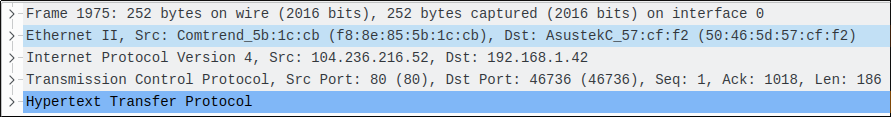
\includegraphics[width=\textwidth]{Resources/Wireshark01.png}
\caption[Captura de pantalla de Wireshark]{Captura de pantalla de Wireshark (Véase \ref{wireshark}, pg. \pageref{wireshark}) en la que se muestran los protocolos que forman un paquete de red HTTP.}
\end{figure}

\subsection{Familia de protocolos de internet}
También conocido como \textit{Internet Protocol Suite}, y más conocido como TCP/IP, es el fundamento de las redes informáticas. Se trata de un conjunto de más de 100 protocolos que permiten la conexión de ordenadores tanto en Internet como en LAN, incluyendo protocolos de las aplicaciones más usadas.

\subsubsection{Aplicación}
Es la capa en la que se envían los datos a otras aplicaciones en otro ordenador o en el mismo. Las aplicaciones hacen uso de las capas inferiores para asegurarse que los datos lleguen a su destino. Algunos de los protocolos más usados son:
\begin{description}
\item \textbf{HTTP} \textit{Hypertex Transfer Protocol:} Protocolo de Transferencia de Hipertexto. Es el protocolo base de la World Wide Web. Se trata de texto estructurado que usa hiperenlaces entre nodos que también contienen texto. El cliente, al entrar en una \acr{url}, el agente de usuario (navegador) envía al servidor una petición de la página web, mediante HTTP. El servidor, envía como respuesta un documento HTML u otro recurso.
\item \textbf{DNS} \textit{Domain Name System:} Sistema de Nombres de Dominio. Un servidor DNS almacena una base de datos distribuida y jerárquica con información sobre el nombre del dominio y la dirección IP a la que está vinculada. Al intentar conectar a  \texttt{http://www.4chan.org}, el cliente pregunta al servidor cual es la dirección IP asociada a esa dirección, y se conecta a tal IP, en este caso 104.16.66.203. Para evitar tener que consultar continuamente con el servidor, se almacenan en una \gls{cache} en el cliente.
\item \textbf{TLS/SSL} \textit{Transport Layer Security}, y su predecesor \textit{Secure Sockets Layer}. <VER APARTADO DE SEGURIDAD>
\item \textbf{HTTPS} HTTP Seguro. Es HTTP con TLS aplicado.
\item \textbf{DHCP} \textit{Dynamic Host Configuration Protocol}: Protocolo de configuración dinámica del host. Este protocolo es controlado por un servidor DHCP que envía parámetros de configuración automática a los clientes. El ejemplo más común es el de cualquier Router doméstico, que asigna automáticamente a cada dispositivo una dirección IP diferente, pero dejando un rango en el que se pueden establecer IP's estáticas.
\item \textbf{FTP} \textit{File Transfer Protocol:} Protocolo de Transferencia de Archivos, te permite enviar archivos entre un cliente y un servidor. El protocolo TLS aplicado a FTP se denomina FTPS. Te permite acceder, mediante un usuario y contraseña, o de forma anónima, a un sistema de archivos jerárquico con nombres de archivo codificados. Utiliza el puerto 21 de forma predeterminada.
\item \textbf{SSH} \textit{Secure Shell:} Terminal seguro. Es un protocolo de red criptográfico que permite a un cliente conectarse a un servidor y ejecutar comandos de terminal como un usuario (conociendo el usuario y contraseña). Además, permite la creación de túneles, lo que permite asegurar cualquier aplicación a través de SSH, y el acceso a puertos bloqueados por el cortafuegos en el cliente. La mayoría de servidores de SSH incluyen un servidor de SFTP, el protocolo FTP con SSH aplicado.
\item \textbf{IMAP} \textit{Internet Message Access Protocol:} Protocolo de acceso a mensajes de Internet. Usa una conexión TCP/IP para conectarse a un servidor de e-mail y ver el contenido de los mensajes, sin necesidad de descargarlos. A diferencia de POP, te permite usar una bandeja de entrada desde varios clientes.
\end{description}
DHCP, DNS, FTP, HTTP, IMAP, POP, TLS/SSL, SMTP, RIP, SSH, Telnet
\subsubsection{Transporte}
\begin{description}
\item \textbf{TCP} \textit{Transmission Control Protocol:} Protocolo de Control de Transmisión. Se aplica a los paquetes para administrarles un orden y un sistema de comprobación de errores. Con todas las funcionalidades, ocupa bastante espacio, lo que aumenta la latencia, aunque es más fiable para el envío de la mayoría de los datos.
\item \textbf{UDP} \textit{User Datagram Protocol:} Es un protocolo muy minimalista. A diferencia del TCP, no garantiza que los paquetes lleguen, o lleguen en orden, o protección ante duplicados. Reduce mucho la latencia ya que no usa \textit{handshaking}. Por ello es usado por ejemplo para \textit{streamings} de televisión o videollamadas.
\end{description}
\subsubsection{Red}
\begin{description}
\item \textbf{IP} \textit{Internet Protocol}: Protocolo de Internet. Envía datagramas o paquetes de red a través de redes. Tiene una función de enrutamiento que es la que permite la interconexión de redes, y la existencia de Internet. Es un protocolo que encapsula el paquete definiendo en el \textit{header} (cabecera) las direcciones IP del servidor y el cliente, o remitente y destinatario. La versión usada actualmente es IPv4 desarrollado en 1981, pero poco a poco se va abriendo paso la versión IPv6. La mayor diferencia es que la versión cuatro cuenta con direcciones de 32 bits lo que permite tan sólo unas 4.3 millardos ($2^{32}$) de direcciones, mientras que la versión 6 tiene direcciones de 128 bits, lo que permite más de 340 sextillones ($2^{128}$)de direcciones
\item \textbf{ICMP} \textit{Internect Control Message Protocol}: Es un protocolo que no es usado por aplicaciones de usuario (a excepción de herramientas de diagnóstico como ping o traceroute). Lo usan los dispositivos de red, como los routers, para enviar notificaciones o mensajes de error indicando que un servicio no está disponible.
\end{description}
\subsubsection{Link}
\begin{description}
\item \textbf{ARP} \textit{Address Resolution Protocol:} Protocolo de resolución de direcciones. Es un protocolo que convierte direcciones de la capa de Red a la capa de Enlace (dir. IP a dir. MAC). 
%\item \textbf{MAC} \textit{Media access control}: Control de acceso al medio. 
\end{description}
ARP, MAC, ETHERNET

\section{Seguridad de redes}
La seguridad de redes consiste en el conjunto de acciones que toma el administrador de redes para prevenir y evitar acceso no autorizado, mal uso, o caída del servicio de red.
\subsection{Tipos de ataques}
Hay dos tipos de ataques de red. Son ataques pasivos cuando el intruso intercepta los datos que viajan por la red, y se considera activo cuando el atacante modifica el funcionamiento normal de la red. Aquí algunos ejemplos de los ataques más comunes:

\begin{easylist}[itemize]
\ListProperties(Style*=$\bullet$ , Style2*=--)
& \textbf{Ataques pasivos}
&& \textbf{Sniffing o analizador de paquetes:} Mediante un software se muestran los datos de los paquetes de red enviados y recibidos por la red.
&& \textbf{Escáner de puertos:} Se envían numerosas peticiones al servidor por los servidores más comunes, así se comprueba que puertos están abiertos. Por ello es recomendable cambiar los puertos por defecto de los servidores importantes.
&& \textbf{Escáner IDLE:} Se realiza un escáner de puertos para saber que servicios están disponibles, pero a traves de otro ordenador "zombie", y observando el comportamiento de éste.
& \textbf{Ataques activos}
&& \textbf{Ataque de Denegación de Servicio:} Se ``desborda" el ancho de banda mediante el envío de muchas peticiones a un servidor, además de ser de un tamaño excesivo.
&& \textbf{Ataque DDoS:} \textit{Distributed Denial of Service}, o un ataque de Denegación de Servicio distribuido. Varios ordenadores hacen un ataque DoS a un mismo servidor, algunas veces los ordenadores forman parte de una \gls{botnet}, y en ocasiones ocurre sin querer (al haber demasiado tráfico de red).
&& \textbf{Phishing:} Con el objetivo de obtener información como nombres de usuario y contraseña o tarjetas de crédito, se crea una página de apariencia parecida a la página que trata de simular. Los usuarios más incautos no notarán el cambio e introducirán sus datos en esta página.
&& \textbf{SQL Injection:} Es una técnica de inserción de código. Al pedir un servidor SQL datos como ``Nombre`` o ``Apellido``, se introduce junto a estos código malicioso que el servidor puede ejecutar. Por ejemplo, \mintinline[breaklines]{SQL}|SELECT * FROM alumnos WHERE nombre = '<nombreintroducido>' ;|. <nombreintroducido> puede ser \texttt{Pablo} o \texttt{Juan}, pero si se introduce \texttt{x'}\mintinline[breaklines]{SQL}|; DROP TABLE alumnos; SELECT * FROM asignaturas WHERE 't' = 't'|, el código que interpreta el servidor eliminaría la tabla \texttt{alumnos} por completo.
&& \textbf{Ataque Smurf:} Es una especie de ataque DDoS. Se envían paquetes ICMP (probablemente pings) a distintas máquinas, pero estos paquetes que se envían, el valor de la dirección IP del remitente es la dirección IP del objetivo al que se quiere atacar. Por lo que, las máquinas a las que se las ha enviado el mensaje ICMP responderán todas al objetivo, haciendo así un DDoS.
&& \textbf{DNS poisoning:} Se modifica la caché de DNS de un ordenador, redireccionando a una IP incorrecta, de esta manera se puede realizar un ataque de phishing sin que lo sepa el usuario del ordenador. En el caso de hacerlo con las tablas de ARP, se denomina \textit{ARP Poisoning}.
\end{easylist}
\subsection{Contramedidas}
\subsubsection{Encriptación}
Se suele denominar también E2EE o \textit{End-to-end encryption}, es decir, encriptación de punto a punto. Se suelen usar claves PGP (\textit{Pretty Good Privacy}, Privacidad bastante buena) para cifrar correos electrónicos y otros archivos. Para HTTP lo más común es la encriptación TLS, aunque también se está utilizando actualmente para email.
\subsubsection{Cortafuegos}
Primero necesitamos definir lo que es un \textbf{puerto}. Un puerto es un punto final de comunicación en un Sistema Operativo. El puerto siempre está asociado a una dirección IP y a un tipo de protocolo. Así completa el origen o destino de un paquete de red. Se aplica en la capa de transporte del modelo OSI. El puerto es un número de 16 bits, por lo que será un número comprendido entre 0 y 65536. Multitud de puertos están ya reservados por diversos protocolos y programas, como el 80 para HTTP, 22 para SSH o 25 para SMTP.

Un cortafuegos es un software que supervisa el tráfico de entrada y salida de datos, basado en unas reglas. Si un paquete de red cumple esas reglas, es rechazado. Pueden bloquear un paquete destinado a un puerto, de un protocolo (Bloquear SSH de Internet, pero no local), de una IP específica, entre otros atributos. También pueden configurarse en modo negativo o whitelist, aceptando tan sólo los paquetes que cumplan las reglas. Por ejemplo, puedes especificar que no acepte tráfico en el puerto 23. Pero igualmente puedes especificar que sólo acepte tráfico en el puerto 23.

\begin{figure}[H]
\noindent
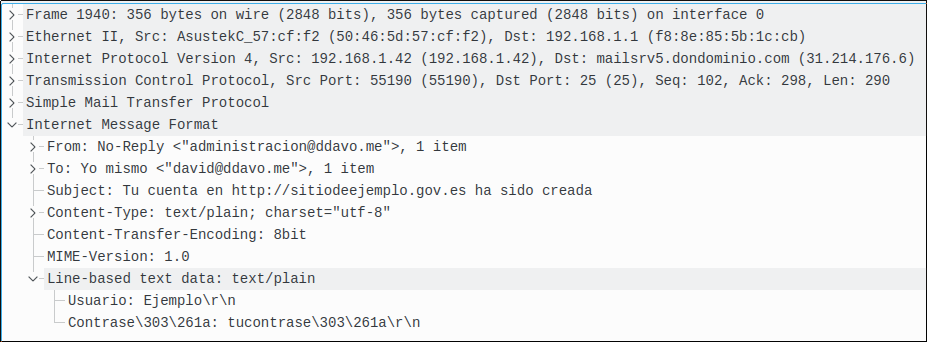
\includegraphics[width=\textwidth]{Resources/Wireshark02.png}
\caption[Wireshark: SMTP sin encriptación]{Captura de pantalla de Wireshark (Véase \ref{wireshark}, pg. \pageref{wireshark}) en la que se muestra un paquete SMTP (email enviado) sin ningún tipo de encriptación. Se puede acceder a este paquete desde cualquier nodo de la red.}
\end{figure}
\begin{figure}[H]
\noindent
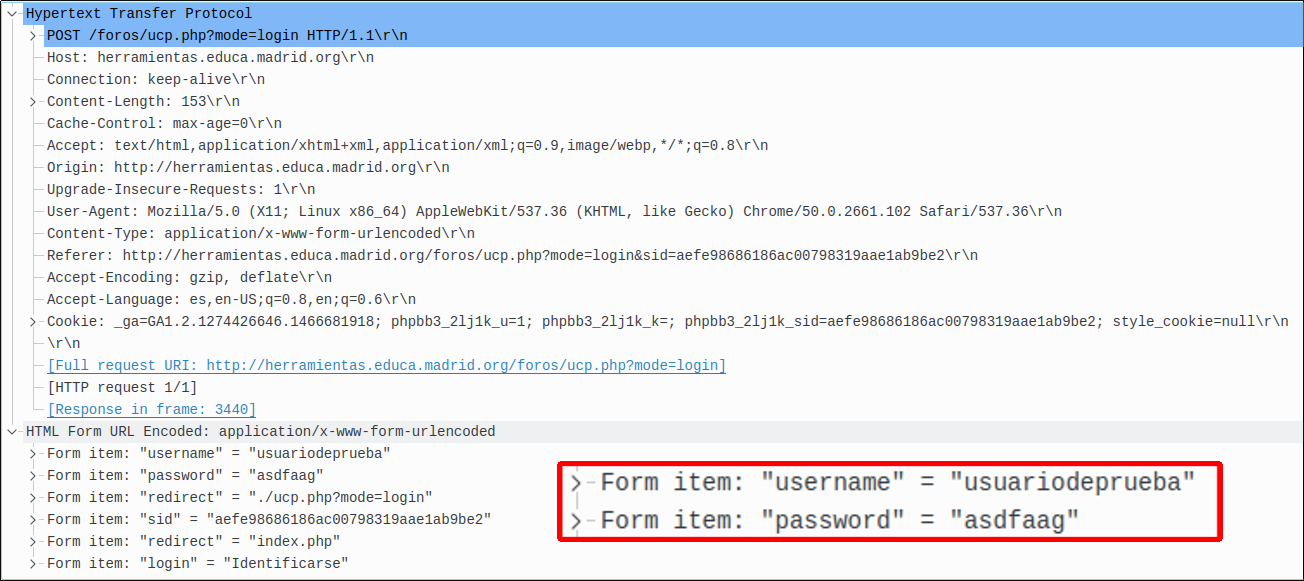
\includegraphics[width=\textwidth]{Resources/Wireshark03.png}
\caption[Wireshark: HTTP Form sin encriptación]{Otro ejemplo de captura de paquetes. Esta vez de un formulario de HTTP en el que personas autorizadas podrían ver el usuario y la contraseña.}
\end{figure}


\chapter{El simulador de redes}
\section{Instalación}
\subsection{Ubuntu / Debian}
Tan sólo debes descargar el paquete del programa. Para ello usa apt-get:
\mint{bash}|Descargas $ sudo apt-get install invproy|

En caso de no estar en los repositorios, hay que hacerlo manualmente:
\begin{minted}{bash}
Descargas $ wget <url>
Descargas $ sudo dpkg -i InvProy.deb
Descargas $ invproy
\end{minted}
Para iniciar el programa también puedes usar la lista de programas.

\subsection{Arch Linux}
Puedes encontrar el programa en el AUR <ENLACE>, pero si nunca has instalado nada desde el AUR, debes seguir el siguiente procedimiento.
\begin{minted}{bash}
~ $ sudo pacman -S base-devel #Lo necesitas para compilar el paquete
#Ahora elige el sitio donde descargaras el paquete. Aqui no se va a instalar.
~ $ cd Builds
Builds $ curl -O <url> #Lo descargamos
Builds $ tar -xvzf invproy.tar.gz
Builds $ cd invproy
Invproy $ makepkg -sri
\end{minted}

Y ya lo tendrías instalado en tu ordenador.

\subsection{Ejecución manual / instalación portable}
Lo primero que necesitarás es descargar las dependencias. Esto depende de el Sistema Operativo. En el caso de GNU/Linux, sólo es necesario descargar \texttt{python3-gobject}. Después, clonamos el repositorio de git. Ejemplo en Ubuntu:
\begin{minted}{bash}
~ $ sudo apt-get update && sudo apt-get upgrade
~ $ sudo apt-get install git python3-gobject
~ $ cd Descargas
Descargas $ git clone https://github.com/daviddavo/InvProy.git
\end{minted}

\noindent Una vez ya tenemos el repositorio de git clonado:
\begin{minted}{bash}
Descargas $ cd InvProy
Descargas $ python3 Main.py
\end{minted}

En el caso de querer usar el programa con una interfaz gráfica, vamos con nuestro explorador de archivos a la carpeta donde queramos descargarlo. Abrimos una terminal y descargamos el programa con \mintinline{bash}|git clone https://github.com/daviddavo/InvProy.git|. Luego entramos en la carpeta y ejecutamos el archivo \texttt{Main.py}
\section{Uso del programa}



\glsaddall
\renewcommand{\glsnamefont}[1]{\makefirstuc{#1}}
\printglossary[style=mcolindex, title=Glosario y acrónimos, toctitle=Glosario y acrónimos]

\nocite{*}
\printbibliography

\listoffigures

\appendix
\chapter{Unidades de transferencia de datos}
Cantidad de datos transferidos por unidad de tiempo. La unidad de tiempo es el segundo y la cantidad de datos puede ser medida en \textit{\glspl{bit}} (bitrate), carácteres/símbolos (\textit{baudrate}) o bytes (8 bits), en ocasiones también se utilizan \textit{nibbles} (4 bits). Para expresar esta velocidad, se suelen usar múltiplos, que pueden ser en base binaria o decimal.

Se usa la ``b" para designar los bits, y ``B" para los Bytes. Después, se usan los prefijos del sistema internacional cuando es en base decimal, y los prefijos del SI cambiando la segunda sílaba por ``bi" (e.g: kilobit / kibibit, kbit/s / Kibit/s) cuando se trata de múltiplos binarios.

\section*{Tabla de múltiplos}
\noindent
\begin{tabularx}{\columnwidth}{| X >{\centering}X X|}
\rowcolor{header} \hline
\textbf{Unidad} & \textbf{Símbolo} & \textbf{Equivalencia} \\ \hline
Kilobit/s & kbit/s o kb/s & 1000 bit/s \\
Megabit/s & Mbit/s o Mb/s & $10^{6}$ bit/s o 10³ kbit/s  \\
Gigabit/s & Gbit/s o Gb/s & $10^{9}$ bit/s o 10³ Mb/s \\
Terabit/s & Tbit/s o TB/s & $10^{12}$ bit/s o 10³ Gb/s \\ \hline
Kibibit/s & Kibit/s & $2^{10}$ bit/s o 1024 bit/s \\
Mebibit/s & Mibit/s & $2^{20}$ bit/s o 1024 Kibit/s \\
Gibibit/s & Gibit/s & $2^{30}$ bit/s o 1024 Mibit/s \\
Tebibit/s & Tibit/s & $2^{40}$ bit/s o 1024 Gibit/s \\ \hline \hline
Byte/s    & Byte/s & 8 bit/s \\
Kilobyte/s & kB/s & 1000 Byte/s o 8000 bits/s \\
Megabyte/s & MB/s & $10^{6}$ Byte/s o 1000 kB/s \\
Gigabyte/s & GB/s & $10^{9}$ Byte/s o 1000 MB/s \\
Terabyte/s & TB/s & $10^{12}$ Byte/s o 1000 GB/s \\ \hline
Kibibyte/s & KiB/s & 1024 Byte/s \\
Mebibyte/s & MiB/s & $2^{20}$ Byte/s \\
Gibibyte/s & GiB/s & $2^{30}$ Byte/s \\
Tebibyte/s & TiB/s & $2^{40}$ Byte/s \\ \hline
\end{tabularx}

\chapter{Código del programa}
%\begin{listing}
\newcommand{\ipm}[1]{
	\section{#1}
	\inputminted[baselinestretch=1, fontsize=\tiny, linenos, breaklines]{python}{Codigo/#1}
}
\ipm{Main.py}
\ipm{Modules/logmod.py}
\ipm{Modules/save.py}
%\section{Interface2.glade} \inputminted[baselinestretch=1, fontsize=\scriptsize, linenos, breaklines]{XML}{Codigo/Interface2.glade}

%\end{listing}

\newpage
\thispagestyle{empty}
\topskip0pt
\vspace*{\fill}
\doclicenseThis
\vspace*{\fill}
\end{document}
